\subsection{Data and Monte Carlo Statistical Uncertainties}

These uncertainties will be computed via bootstrapping.  A set of $N$ pseudodatasets are performed where each event has a weight $W_\text{pseudo}w_\text{nominal}$, where $w_\text{nominal}$ is one for data and $w_\text{MC}$ for simulation; $W_\text{pseudo}$ is a Poisson random variable that has a new value for each pseudodataset and has a mean of one.  To ensure that the uncertainty on the uncertainty is negligible, $N\gtrsim 100$.  These uncertainties are straightforward to compute, but are computationally expensive and thus we will compute them once all other results are finished.

\subsection{Pileup reweighting uncertainties}
As discussed in section~\ref{subsec:PRW}, a correction is applied to MC events such that the pileup modeling in the simulation corresponds to what is seen in data. As such, there are variations associated with this modeling
that must be taken into account.

In addition, a scaling correction is applied to the data during pileup reweighting. Nominally, this scaling correction is equal to 1/1.03, and the up and down variations are set to 1/1.072 and 1/1.35 respectively.

\subsection{Muon uncertainties}

\subsubsection{Muon efficiency uncertainties}
As summarized in section~\ref{subsec:MCCorr} there are several scale factors associated with muon reconstruction related to efficiencies in the trigger, reconstruction, isolation and track-to-vertex association.
Hence, there are 2 systematic variations associated with the trigger efficiency, 2 for the isolation efficiency, 4 for the reconstruction efficiency, and 2 for the TTVA efficiency:
\begin{itemize}
  \item MUON\_EFF\_TrigSystUncertainty
  \item MUON\_EFF\_TrigStatUncertainty
  \item MUON\_EFF\_ISO\_SYS
  \item MUON\_EFF\_ISO\_STAT
  \item MUON\_EFF\_RECO\_SYS
  \item MUON\_EFF\_RECO\_SYS\_LOWPT
  \item MUON\_EFF\_RECO\_STAT
  \item MUON\_EFF\_RECO\_STAT\_LOWPT
  \item MUON\_EFF\_TTVA\_SYS
  \item MUON\_EFF\_TTVA\_STAT
\end{itemize}

The impact of the efficiency systematics is summarized in figure~\ref{fig:PP8SFSyst}.

\begin{figure}[h!]
  \centering
  \subfloat[MC16a]{\includegraphics[page=2,width=\textwidth]{figures/ZjetOmnifoldSystematics.pdf}} \\
  \subfloat[MC16d]{\includegraphics[page=9,width=\textwidth]{figures/ZjetOmnifoldSystematics.pdf}} \\
  \subfloat[MC16e]{\includegraphics[page=16,width=\textwidth]{figures/ZjetOmnifoldSystematics.pdf}} \\
  \subfloat[Run 2]{\includegraphics[page=22,width=\textwidth]{figures/ZjetOmnifoldSystematics.pdf}}
  \caption{The fractional systematic impact for the pileup efficiency and the muon efficiencies for the \powheg+\pythia~samples across all years as a function of the dilepton \pt. The upwards shift is presented in red, and the downwards shift in blue.}
  \label{fig:PP8SFSyst}
\end{figure}

\subsubsection{Muon calibration uncertainties}
There are also systematic variations associated with the calibration applied to the muons. These will have an affect on the muon kinematics. The systematic variations are listed below, and include
one for momentum variations due to measurements made in the inner detector, one for momentum effects related to the muon spectrometer, one for the momentum scale, and 2 systematics related to the measured sagitta value.
\begin{itemize}
  \item MUON\_ID (inner detector track resolution)
  \item MUON\_MS (muon spectrometer track resolution)
  \item MUON\_SCALE (momentum scale)
  \item MUON\_SAGITTA\_RESBIAS (residual bias correction)
  \item MUON\_SAGITTA\_RHO (combined measurement correction)
\end{itemize}

The effects of these variations are shown in figure~\ref{fig:PP8MuCalSyst}.

\begin{figure}[h!]
  \centering
  \subfloat{\includegraphics[page=5,width=\textwidth]{figures/ZjetOmnifoldSystematics.pdf}} \\
  \subfloat{\includegraphics[page=12,width=\textwidth]{figures/ZjetOmnifoldSystematics.pdf}} \\
  \subfloat{\includegraphics[page=19,width=\textwidth]{figures/ZjetOmnifoldSystematics.pdf}} \\
  \subfloat{\includegraphics[page=25,width=\textwidth]{figures/ZjetOmnifoldSystematics.pdf}}
  \caption{The fractional systematic impact for variations to the muon calibration for the \powheg+\pythia~samples for all years as a function of the dilepton \pt. The upwards shift is presented in red, and the downwards shift in blue.}
  \label{fig:PP8MuCalSyst}
\end{figure}

\subsection{Track uncertainties}

The systematic uncertainties associated with the tracks are:

\begin{itemize}
  \item InDet::TRK\_EFF\_TIGHT\_GLOBAL
  \item InDet::TRK\_EFF\_TIGHT\_IBL
  \item InDet::TRK\_EFF\_TIGHT\_PP0
  \item InDet::TRK\_EFF\_TIGHT\_PHYSMODEL
  \item InDet::TRK\_EFF\_LOOSE\_TIDE
  \item InDet::TRK\_FAKE\_RATE\_LOOSE
  \item InDet::TRK\_BIAS\_QOVERP\_SAGITTA\_WM
\end{itemize}

The first four are combined into one nuisance parameter and are due to variations of the tracking efficiency. The fifth describes the variations to the tracking efficiency when the track is inside a jet.
The sixth represents variations to the fake rate. The last varies the \pt of the track based on the residual alignment uncertainties.

\begin{figure}[h!]
  \centering
  \subfloat[MC16a]{\includegraphics[page=7,width=0.45\textwidth]{figures/ZjetOmnifoldSystematics.pdf}}
  \subfloat[MC16d]{\includegraphics[page=14,width=0.45\textwidth]{figures/ZjetOmnifoldSystematics.pdf}} \\
  \subfloat[MC16e]{\includegraphics[page=21,width=0.45\textwidth]{figures/ZjetOmnifoldSystematics.pdf}}
  \subfloat[Run 2]{\includegraphics[page=27,width=0.45\textwidth]{figures/ZjetOmnifoldSystematics.pdf}}
  \caption{The fractional systematic impact for variations applied to the tracks for the \powheg+\pythia~samples for all years. Note that only the down variations are shown for the inclusive efficiency, inside jet efficiency and the fake rate.
  The variations are symmetrized for use in the analysis.}
  \label{fig:PP8TrackSyst}
\end{figure}

\subsection{Modeling and unfolding uncertainties}

Modeling uncertainties are determined by unfolding the data with simulations that have different physics models.  We will do this by first comparing the result when unfolding with \pythia and when unfolding with \sherpa.  This is a crude uncertainty because there are multiple differences between these generators.  We will supplement this comparison by unfolding with various \powheg+\pythia samples that have been re-weighted based on truth-level samples that have targeted variations (e.g. A14 tune variations).  Additional samples are being prepared by the PMG but will likely not be ready in time for this analysis.

Unfolding uncertainties are designed to quantify the method closure.  We will do this by unfolding \pythia with \sherpa and then comparing to the \pythia truth (and vice versa).  This may have some double-counting with modeling uncertainties and is often mitigated by performing some reweighting\footnote{\url{https://twiki.cern.ch/twiki/bin/viewauth/AtlasProtected/StandardModelUnfolding}}~\cite{Malaescu:2009dm} (which actually is similar to OmniFold Step 1).  However, we will choose the more conservative approach for this first high-dimensional analysis.


\subsection{Theoretical uncertainties}
\subsubsection{QCD renormalization and factorization scale variations}
The variation of the QCD renormalization ($\mu_r$) and factorization ($\mu_f$) scale on the process was studied using the \sherpa\ event generator. This generator can vary each scale independently and provides combinations of up (2$\mu_(r,f)$) and down (0.5$\mu_(r,f)$) variations of each scale. The impact of these scale variations is shown in figure~\ref{fig:QCDscale_mjj}, increasing the scales results in less events in the observed dilepton \pt spectrum and vice versa.
\begin{figure}[h!]
  \centering
  \subfloat[MC16a]{\includegraphics[page=2,width=0.45\textwidth]{figures/systQCD.pdf}}
  \subfloat[MC16d]{\includegraphics[page=4,width=0.45\textwidth]{figures/systQCD.pdf}} \\
  \subfloat[MC16e]{\includegraphics[page=6,width=0.45\textwidth]{figures/systQCD.pdf}}
  \subfloat[Run 2]{\includegraphics[page=7,width=0.45\textwidth]{figures/systQCD.pdf}}
  \caption{The fractional impact of the QCD scale variations for the \sherpa~samples on the dilepton \pt spectrum for all the years and full Run2. The result of varying $\mu_r$ and $\mu_f$ in the up direction is shown in red and the downwards shift is in blue.}
  \label{fig:QCDscale_mjj}
\end{figure}

%\subsubsection{Parton Distribution Function (PDF) variations}


